\section{\model: Role Specialization}

Assigning LLM agents clear, well-defined roles with specific goals enables the breakdown of complex objectives into smaller, manageable subtasks. Financial trading is a prime example of such complexity, demanding the integration of diverse signals, inputs, and specialized expertise. In the real world, this approach to managing complexity is demonstrated by trading firms that rely on expert teams to collaborate and make high-stakes decisions, underscoring the multifaceted nature of the task.

In a typical trading firm, vast amounts of data are collected, including financial metrics, price movements, trading volumes, historical performance, economic indicators, and news sentiment. This data is then analyzed by quantitative experts (quants), including mathematicians, data scientists, and engineers, using advanced tools and algorithms to identify trends and predict market movements.

Inspired by this organizational structure, \model defines seven distinct agent roles within a simulated trading firm: Fundamentals Analyst, Sentiment Analyst, News Analyst, Technical Analyst, Researcher, Trader, and Risk Manager. Each agent is assigned a specific name, role, goal, and set of constraints, alongside predefined context, skills, and tools tailored to their function. For example, a Sentiment Analyst is equipped with tools like web search engines, Reddit search APIs, X/Twitter search tools, and sentiment score calculation algorithms, while a Technical Analyst can execute code, calculate technical indicators, and analyze trading patterns. More specifically, \model assumes the following teams.



\subsection{Analyst Team}

The Analyst Team (Figure \ref{fig:analyst}) is composed of specialized agents responsible for gathering and analyzing various types of market data to inform trading decisions. Each agent focuses on a specific aspect of market analysis, bringing together a comprehensive view of the market's conditions.

\begin{figure}[htbp]
\centerline{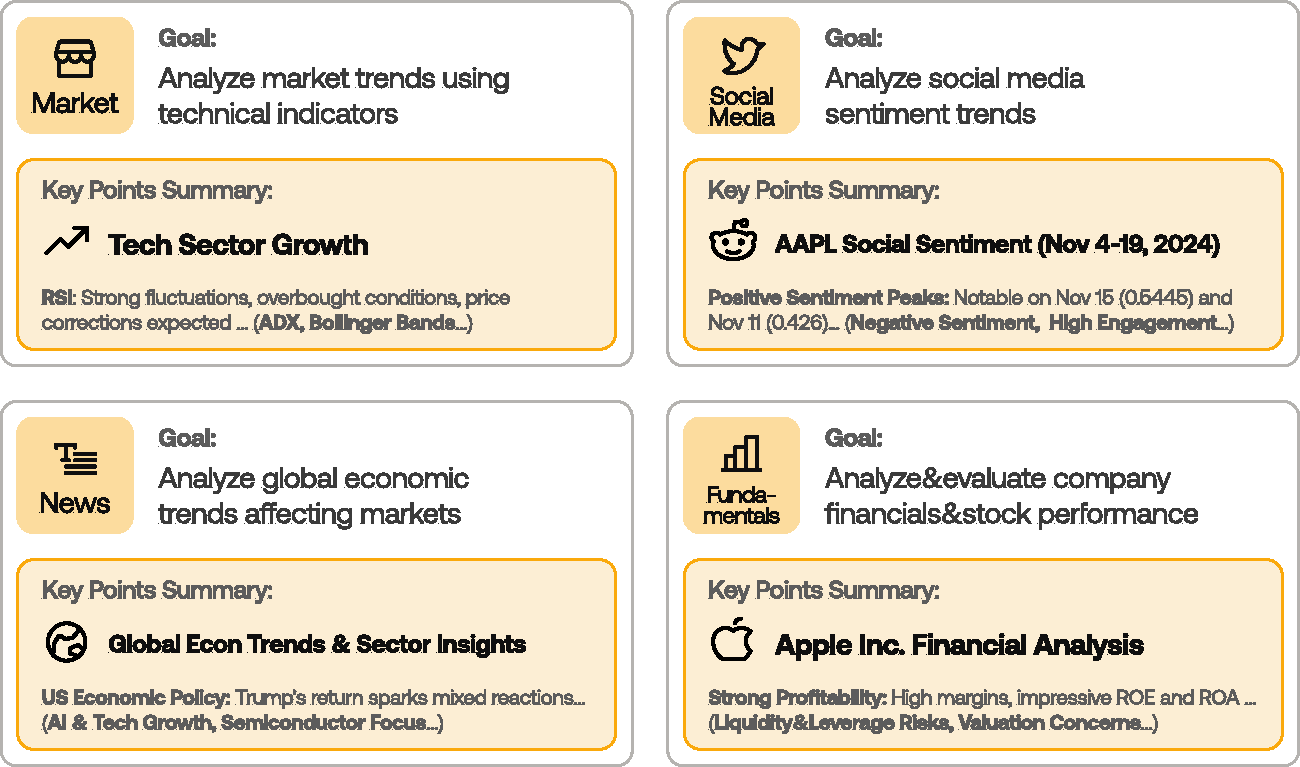
\includegraphics[width=0.9\linewidth]{figures/analyst.pdf}}
\caption{\model Analyst Team}

\label{fig:analyst}
\end{figure}

\begin{itemize}
    \item \textbf{Fundamental Analyst Agents}: These agents evaluate company fundamentals by analyzing financial statements, earnings reports, insider transactions, and other pertinent data. They assess a company's intrinsic value to identify undervalued or overvalued stocks, providing insights into long-term investment potential.
    \item \textbf{Sentiment Analyst Agents}: These agents process large volumes of social media posts, sentiment scores, and insider sentiments derived from public information and social media activity. They gauge market sentiment to predict how collective investor behavior might impact stock prices in the short term.
    \item \textbf{News Analyst Agents}: These agents analyze news articles, government announcements, and other macroeconomic indicators to assess the market's macroeconomic state, major world events, and significant company changes. They identify news events that could influence market movements, helping to anticipate sudden shifts in market dynamics.
    \item \textbf{Technical Analyst Agents}: These agents calculate and select relevant technical indicators, such as Moving Average Convergence Divergence (MACD) and Relative Strength Index (RSI), customized for specific assets. They analyze price patterns and trading volumes to forecast future price movements, assisting in timing entry and exit points.
\end{itemize}


Collectively, the Analyst Team synthesizes data from multiple sources to provide a holistic market analysis. Their combined insights form the foundational input for the Researcher Team, ensuring that all facets of the market are considered in subsequent decision-making processes.


\subsection{Researcher Team}

The Researcher Team (Figure \ref{fig:researcher}) is responsible for critically evaluating the information provided by the Analyst Team. Comprised of agents adopting both bullish and bearish perspectives, they engage in multiple rounds of debate to assess the potential risks and benefits of investment decisions.

\begin{figure}[htbp]
\centerline{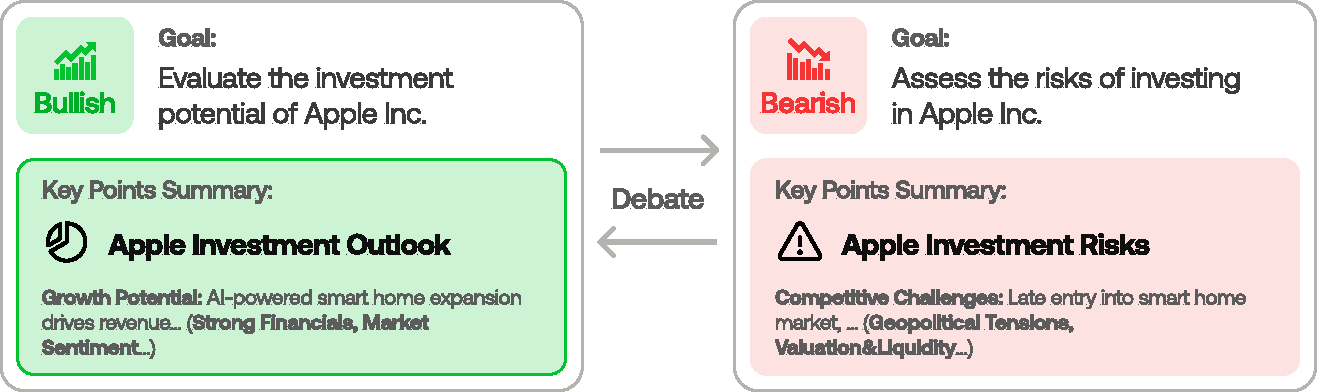
\includegraphics[width=0.9\linewidth]{figures/researcher.pdf}}
\caption{\model Researcher Team: Bullish Perspectives and Bearish Perspectives}
\label{fig:researcher}
\end{figure}


\begin{itemize}
    \item \textbf{Bullish Researchers}: These agents advocate for investment opportunities by highlighting positive indicators, growth potential, and favorable market conditions. They construct arguments supporting the initiation or continuation of positions in certain assets.
    \item \textbf{Bearish Researchers}: Conversely, these agents focus on potential downsides, risks, and unfavorable market signals. They provide cautionary insights, questioning the viability of investment strategies and highlighting possible negative outcomes.
\end{itemize}


Through this dialectical process, the Researcher Team aims to reach a balanced understanding of the market situation. Their thorough analysis helps in identifying the most promising investment strategies while anticipating possible challenges, thus aiding the Trader Agents in making informed decisions.




\subsection{Trader Agents}

Trader Agents (Figure \ref{fig:trader}) are responsible for executing trading decisions based on the comprehensive analysis provided by the Analyst Team and the nuanced perspectives from the Researcher Team. They assess the synthesized information, considering both quantitative data and qualitative insights, to determine optimal trading actions.

\begin{figure}[htbp]
\centerline{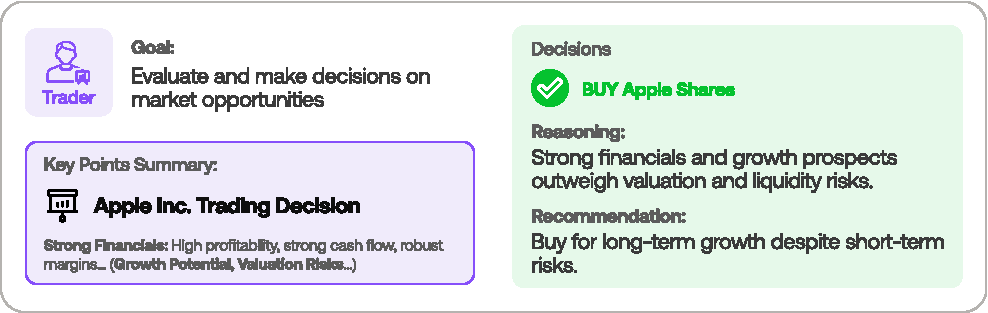
\includegraphics[width=0.9\linewidth]{figures/trader.pdf}}
\caption{\model's Trader Decision-Making Process}
\label{fig:trader}
\end{figure}


The tasks of \model Trader include:

\begin{itemize}
    \item Evaluating recommendations and insights from analysts and researchers.
    \item Deciding on the timing and size of trades to maximize trading returns.
    \item Placing buy or sell orders in the market.
    \item Adjusting portfolio allocations in response to market changes and new information.
\end{itemize}

Trader Agents must balance potential returns against associated risks, making timely decisions in a dynamic market environment. Their actions directly impact the firm's performance, necessitating a high level of precision and strategic thinking.

\subsection{Risk Management Team}

The Risk Management Team (Figure \ref{fig:risk_mgmt}) monitors and controls the firm's exposure to various market risks. These agents continuously evaluate the portfolio's risk profile, ensuring that trading activities remain within predefined risk parameters and comply with regulatory requirements.


The responsibilities of Risk Management Team include:

\begin{itemize}
    \item Assessing factors such as market volatility, liquidity, and counterparty risks.
    \item Implementing risk mitigation strategies, such as setting stop-loss orders or diversifying holdings.
    \item Providing feedback to Trader Agents on risk exposures and suggesting adjustments to trading strategies.
    \item Ensuring that the overall portfolio aligns with the firm's risk tolerance and investment objectives.
\end{itemize}

\begin{figure}[htbp]
\centerline{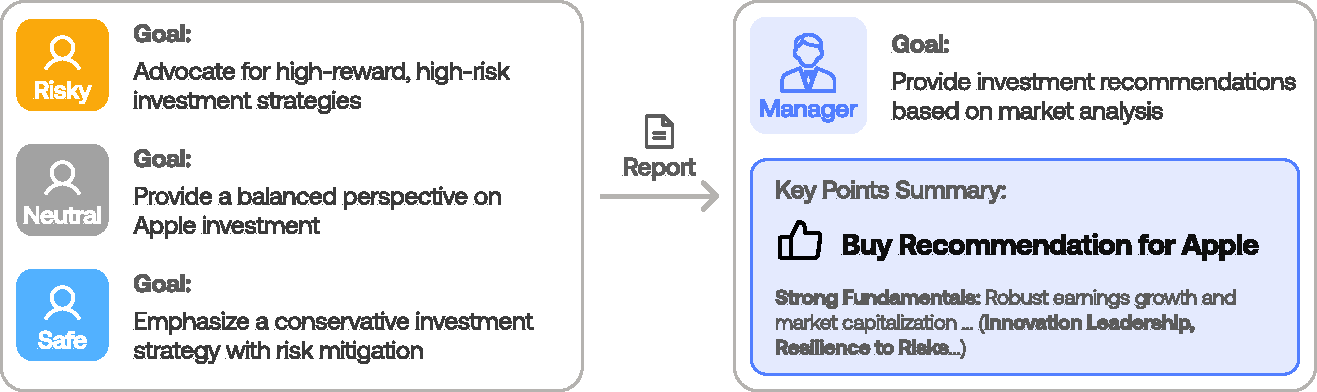
\includegraphics[width=0.9\linewidth]{figures/risk_mgmt.pdf}}
\caption{\model Risk Management Team and Fund Manager Approval Workflow}
\label{fig:risk_mgmt}
\end{figure}


By offering oversight and guidance, the Risk Management Team helps maintain the firm's financial stability and protect against adverse market events. They play a crucial role in safeguarding assets and ensuring sustainable long-term performance.

All agents in \model follow the ReAct prompting framework \citep{yao2023reactsynergizingreasoningacting}, which synergizes reasoning and acting. The environment state is shared and monitored by the agents, enabling them to take context-appropriate actions such as conducting research, executing trades, engaging in debates, or managing risks. This design ensures a collaborative, dynamic decision-making process reflective of real-world trading systems.


\section{\model: Agent Workflow}

\subsection{Communication Protocol}

Most existing LLM-based agent frameworks use natural language as the primary communication interface, typically through structured message histories or collections of agent-generated messages \citep{fatouros2024largelanguagemodelsbeat, li2023tradinggpt, yang2024finrobotopensourceaiagent, yang2023autogptonlinedecisionmaking}. However, relying solely on natural language often proves insufficient for solving complex, long-term tasks that require extensive planning horizons. In such cases, pure natural language communication can resemble a game of telephone—over multiple iterations, initial information may be forgotten or distorted due to context length limitations and an overload of text that obscures critical earlier details \citep{hong2024metagptmetaprogrammingmultiagent}. To address this limitation, we draw inspiration from frameworks like MetaGPT, which adopt a structured approach to communication. Our model introduces a structured communication protocol to govern agent interactions. By clearly defining each agent's state, we ensure that each role only extracts or queries the necessary information, processes it, and returns a completed report. This streamlined approach reduces unnecessary steps, lowers the risk of message corruption, and keeps interactions focused and efficient, even in complex, long-horizon tasks.

\subsection{Types of Agent Interactions}

In contrast to previous multi-agent trading frameworks, which rely heavily on natural language dialogue, \model agents communicate primarily through structured documents and diagrams. These documents encapsulate the agents' insights in concise, well-organized reports that preserve essential content while avoiding irrelevant information. By utilizing structured reports, agents can query necessary details directly from the global state, eliminating the need for lengthy conversations that risk diluting information, extending the message state indefinitely, and causing data loss. The types of documents and the information they contain are detailed below:

% \begin{itemize}
%     \setlength\itemsep{0em}
%     \setlength\leftmargin{0em}
%     \item
\textbf{I. Analyst Team}: Fundamental, sentiment, news, and technical analysts compile their research and findings into concise analysis reports specific to their areas of expertise. These reports include key metrics, insights, and recommendations based on their specialized analyses.

\textbf{II. Traders}: Traders review and analyze the reports from the analysts, carefully deliberating to produce clear decision signals. They accompany these decisions with detailed reports explaining their rationale and supporting evidence, which are later utilized by the risk management team.
% \end{itemize}

Agents engage in natural language dialogue exclusively during agent-to-agent conversations and debates. These concise, focused discussions have been shown to promote deeper reasoning and integrate diverse perspectives, enabling more balanced decisions in complex, long-horizon scenarios—a method particularly relevant to the intricate environment of trading \citep{du2023improvingfactualityreasoninglanguage}. This approach seamlessly integrates with our structured framework, as the conversation state is recorded as a structured entry within the overall agent state. The types of communication in these scenarios are detailed below:



% \begin{itemize}
%     \item
\textbf{III. Researcher Team}: Each researcher agent queries the global agent state for analyst reports and carefully forms their opinion. Two researchers represent opposing perspectives: one bullish and one bearish. They engage in natural language dialogue for $n$ rounds, as determined by the debate facilitator agent. At the conclusion, the facilitator reviews the debate history, selects the prevailing perspective, and records it as a structured entry in the communication protocol.

\textbf{IV. Risk Management Team}: The risk management team, similar to the researcher team, queries the trader's decision and accompanying report. They then deliberate from three perspectives—risk-seeking, neutral, and risk-conservative—to adjust the trading plan within risk constraints. They engage in $n$ rounds of natural language discussion, guided by a facilitator agent.

\textbf{V. Fund manager}: The fund manager reviews the discussion from the risk management team, determines the appropriate risk adjustments, and updates the trader's decision and report states within the communication protocol.
% \end{itemize}


\subsection{Backbone LLMs}

To meet the diverse complexity and speed demands of tasks in our framework, we strategically select Large Language Models (LLMs) based on their strengths. Quick-thinking models, such as \verb|gpt-4o-mini| and \verb|gpt-4o|, efficiently handle fast, low-depth tasks like summarization, data retrieval, and converting tabular data to text \citep{openai2024gpt4technicalreport}. In contrast, deep-thinking models like \verb|o1-preview| excel in reasoning-intensive tasks such as decision-making, evidence-based report writing, and data analysis. These models leverage their architectures for multi-round reasoning, producing logically sound, in-depth insights \citep{zhong2024evaluationopenaio1opportunities, wang2024planningabilitiesopenaiso1, openai2024o1}. Additionally, we prioritize models with proven reliability and scalability to ensure optimal performance across various market conditions. We also employ auxiliary expert models for specialized tasks like sentiment analysis.



Specifically, all analyst nodes rely on deep-thinking models to ensure robust analysis, while quick-thinking models handle data retrieval from APIs and tools for efficiency. Researchers and traders use deep-thinking models to generate valuable insights and support well-informed decisions. By aligning the choice of LLMs with the specific requirements of each task, our framework achieves a balance between efficiency and depth of reasoning, which is crucial for effective trading strategies.


This implementation strategy ensures that \model can be deployed without requiring a GPU, relying only on API credits. It also introduces seamless exchangeability of backbone models, enabling researchers to effortlessly replace the model with any locally hosted or API-accessible alternatives in the future. This adaptability supports the integration of improved reasoning models or finance-tuned models customized for specific tasks. As a result, \model is highly scalable and future-proof, offering flexibility to accommodate any backbone model for any of its agents.
